\chapter{Project Plan}
    This chapter will briefly talk about the 5S Drifter project motivations as well their function as a product developed 
    by the Minho's University under supervision by the professors Luis Gonçalves and Sérgio Lopes.
\section{Introduction}
\label{sec:Introduction}
Under the course unity of Integrative Project in Industrial Electronics and Computers the students must
apply for professors projects in order to integrate unde their respective laboratories and start to undertand the pace
demanded on the Master's final paper.

This project, given by the professor Luis Gonçalves and Sergio Lopes under the CMEMS laboratory,
has the main porpouse to create a drifter for data aquisition. As a multi-themed project, this report will
explore multiple areas, as the PCB design for hardware and firmware manufacture, software design under the idea to optimize
the execution allowing for better performance. The main goal is to have the final product afloat at the end of the simester.

\begin{figure}[H]
    \centering
    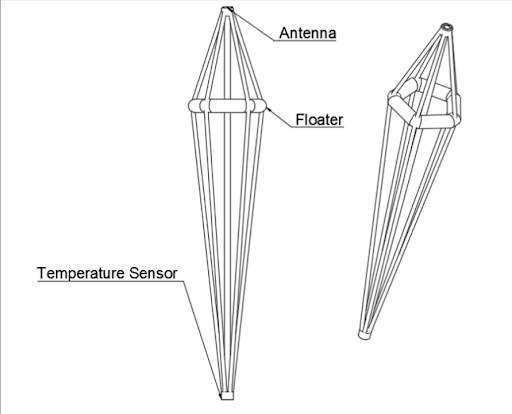
\includegraphics[width=0.7\textwidth]{images/diagrams/shell/unnamed.png}  % Adjust the width as necessary
    \caption{Draft Floater}
    \label{fig:Draft Floater}        
\end{figure}

\subsection{Problem Statement}
\label{sec:Problem Statement}
The ocean is one of the man the greatest mystery even before the written history. Humanity made the world ours over the water, 
from the Portuguese greatest discoveries, braving the raging ocean to the newest oil tanker demanding ever newer technology
in order to tame the sea for safer and smoother sailing.

Nowadays, scientists believe only 20\% to 26\% of the ocean is discovered with the actual technology which means that humanity 
know as much about our so grate sky as our own seas. 5S ocean drifter is equipment made to acquire date from 
superficial sea streams and expand the oceanographic knowledge about it.

Better knowledge of the ocean lead to further development in diverse areas. Granting safety,
security and efficiency.

5S, an acronym for Sensoring System for Surface Sea Streams is a low-cost, low-power solution to acquire
said data with the focus to last autonomously for the longest time possible. The drifter has to attain its GPS
coordinates in order to track its current and average velocity, alongside with the water temperature and an accelerometer 
information to gather information about the wave intensity. All this data will be stored locally and transmitted by a protocol,
yet to be defined, with a JSON format in order to be received by a database that already is implemented.  


\subsubsection{Oceanograpy}
\label{sec:Oceanograpy}
The current in study will be the IPC (Iberian Poleward Current), a well documented by the Advanced Very High Resolution Radiometer (AVHRR)
over the last two decades, is a narrow (25-40km) flow of water that follows the continent slope due to topography and/or water density
commonly referred as a "slope-trapped tongue". Iberian as is "slope-trapped" at the continent going roughly near Portugal going along 
up to the bay of Biscay and Poleward, meaning that the current flows North. Being at their strongest in the winter, and weaker at the summer
peak, the current is known to be significantly warmer and carrying more salinity due to the Mediterranean influence, over the 
Eastern North Atlantic Central Water (ENACW).

\subsubsection{Transport}
It isn't uncommon to see transport accidents being reported, and even worse, for it to be a gigantic problem.
Some of these accidents are caused by poor mapping of sea conditions, tankers spilling oil, fishing vessels capsizing, leading
to financial problems and even loss of life. Even when there are no accidents, poor knowledge of tides results in higher energy consumption when routes are set against the currents.

A solution would be to create optimized shipping routes, minimizing accidents and improving energy efficiency while 
traversing the waves. Oil tankers could follow currents with lower fuel consumption. Fishing routes could become more
efficient, as their target species may swim with the tides based on temperature and speed. This would ease the workload,
making the activity less reactive and more predictable, aligning expected catch rates with reduced time and energy 
consumption.

A well-known example of a hazardous area is the Nazaré Canyon, where its unique shape creates enormous waves. 
Avoiding these waters is crucial for safer navigation.

\subsubsection{Ecology}

The IPC has an important part in their ecosystem, as it transports plankton transport, larval drift, and 
nutrient dynamics along the coast, essential components for the living fauna and flora.


Other way to see the importance of IPC looking after the ecology is the placement of wave energy converters, a 
growing field under the energy generation, is one of the main problems the technology faces. 
A good positioning improves the efficiency and reduces the costs of construction and maintenance.
\begin{figure}[H]
    \centering
    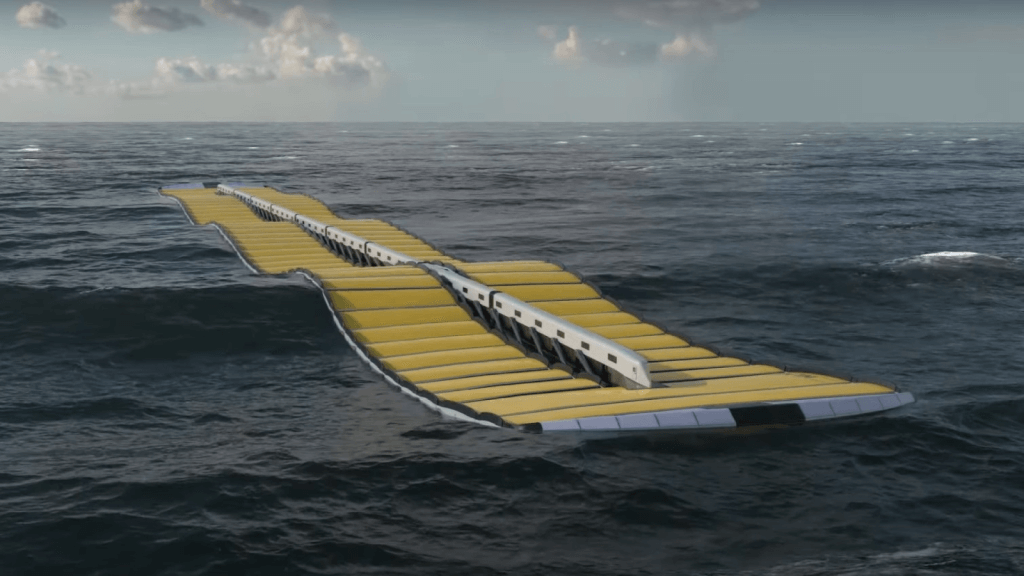
\includegraphics[width=0.7\textwidth]{images/chapter/introduction/renewable_energy.png}  % Adjust the width as necessary
    \caption{The Design of a Wave Energy Converter to Electricity}
    \label{fig:The Design of a Wave Energy Converter to Electricity}        
\end{figure}

Nowadays, the field of renewable energy overseas is a hot topic, as the designs keep on changing and improving. As an example, the company
Ocean Winds builds offshore wind farms over the world. Recently the company created the project WindFloat in Portugal as initiative
to harvest the offshore winds in areas with depth greater than 40 meters, being around a few kilometers.

\begin{figure}[H]
    \centering
    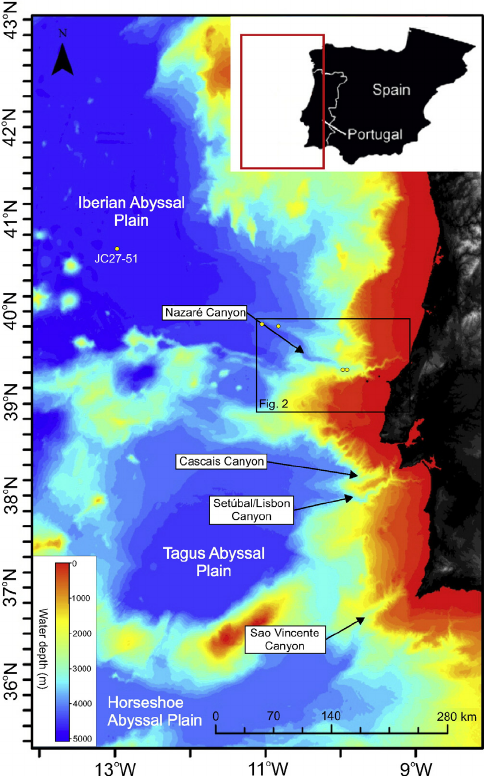
\includegraphics[angle=90,origin=c,width=0.7\textwidth]{images/maps/pt_depth.png}  % Adjust the width as necessary
    \vspace{-2.2cm}
    \caption{Depth Map of Portugal's Coast}
    \label{fig:Depth Map of Portugal's Coast}        
\end{figure}


\subsubsection{Safety}
As time passes one the important jobs of oceanography is the study of sediments of rocky
structures at shore and their deposition. Data useful to determine the shore mineral composition
and predict erosion areas or even weaker or stronger soil helping to plan coastal vulnerability and resilience.

The coast is a focus human attractor, being for sports, leisure, living and Industrial oportunities, and being so, good information around it
prevent harm, and creates a safer environment.   

\subsection{Problem Statement Analysis}
As a first step into solving this project, an initial construction of the
demends is requested. Here will be presented, following the waterfall aprouch
and UML standarts, the solutions to the individual problems presented by the project.

As stated, the floater has a series of data to acuare, format, and send in order to 
be considered concluded. The system will be divided in smaller and simpler packeges to solve
each point then it will be assembled as a final product.

\subsubsection{Equipment Objectives}
The system, in order to acomplish said targets, must set the following topics

\begin{itemize}
    \item Data aquisition
    \begin{itemize}
        \item Power Source Level \\ In order to alert a low batteries.
        \item Wave intensity \\ Measuring the force exercised by the water in the drifter
        \item Position \\ Track the movement of the water.
        \item Temperature \\ Measures the temperature directly.
    \end{itemize}
    \item Wireless data transference \\ As the floaters has no physical connections with the shore. 
    \item Local data storage \\ In case of lack of external communication.
    \item Autonomy \\ The longer it survives, the more data it will gather.
    \item Resistant and buoyant shell \\ The physical parts that support the system.
\end{itemize}





